\section{\large \textcolor{blue}{Interferência, Difração, Refração e Reflexão}}

\begin{flushleft}
\textbf{\textcolor{blue}{\Large Quest\~ao 43}}\\
\noindent
\subsection{Quest\~ao 43 - Filmes Finos}
Luz com 650 nm de comprimento de onda incide
perpendicularmente em um filme fino de sabão, que tem
índice de refração igual a 1,30. Sabendo que esse filme está
suspenso no ar, qual a menor espessura que esse filme
deve ter para que as ondas refletidas por ele sofram
interferência construtiva?

\begin{itemize}
\item[(A)] 320 nm.
\item[(B)] 242 nm.
\item[(C)] 125 nm.
\item[(D)] 117 nm.
\end{itemize}

\vspace{0.5cm}

\textcolor{red}{\textbf{Solução:}}\\

\section*{Interferência construtiva em um filme de sabão}

\textbf{Dados:}
\begin{itemize}
    \item Comprimento de onda no ar: \( \lambda_0 = 650\,\mathrm{nm} \)
    \item Índice de refração do filme: \( n_f = 1{,}30 \)
    \item Índice de refração do ar: \( n_{ar} \approx 1 \)
\end{itemize}

O filme está suspenso no ar. Queremos a menor espessura \(e\) para que a luz refletida tenha interferência construtiva.

\subsection*{Condição de fase}

Quando a luz incide sobre a superfície do filme:
\begin{itemize}
    \item Na interface ar–sabão (\(n_\text{ar} < n_\text{sabão}\)), ocorre inversão de fase de \(\pi\) (equivalente a \(\lambda/2\)).
    \item Na interface sabão–ar (\(n_\text{sabão} > n_\text{ar}\)), não ocorre inversão.
\end{itemize}

Como há uma inversão de fase, a condição para \textbf{interferência construtiva} é:
\[
2e = \left(m + \frac{1}{2}\right) \lambda_f
\]

Para a menor espessura (\(m = 0\)):
\[
2e = \frac{\lambda_f}{2} \quad \implies \quad e = \frac{\lambda_f}{4}
\]

\subsection*{Comprimento de onda no filme}

No interior do filme, o comprimento de onda é menor:
\[
\lambda_f = \frac{\lambda_0}{n_f} = \frac{650}{1{,}30} \approx 500\,\mathrm{nm}
\]

\subsection*{Espessura mínima}

Substituindo:
\[
e_\text{mín} = \frac{\lambda_f}{4} = \frac{500}{4} = 125\,\mathrm{nm}
\]

\subsection*{Resposta final:}
\[
\boxed{e_\text{mín} = 125\,\mathrm{nm}}
\]


A resposta correta é alternativa \colorbox{green!50}{\textbf{C}}.
\end{flushleft}

\noindent\rule{\linewidth}{0.6pt}\\

\section*{Intervalo válido para o comprimento de onda de um laser}

O comprimento de onda (\( \lambda \)) de um laser depende do material ativo utilizado no laser e pode abranger diferentes regiões do espectro eletromagnético. Abaixo estão os intervalos típicos para lasers comuns:

\begin{center}
\begin{tabular}{|l|c|}
\hline
\textbf{Tipo de laser} & \textbf{Comprimento de onda (\( \lambda \))} \\
\hline
Laser ultravioleta (UV) & \(180\,\mathrm{nm} \text{ a } 400\,\mathrm{nm}\) \\
\hline
Laser visível (vermelho-violeta) & \(400\,\mathrm{nm} \text{ a } 700\,\mathrm{nm}\) \\
\hline
Laser infravermelho próximo (NIR) & \(700\,\mathrm{nm} \text{ a } 1400\,\mathrm{nm}\) \\
\hline
Laser infravermelho médio & \(1400\,\mathrm{nm} \text{ a } 3000\,\mathrm{nm}\) \\
\hline
Laser infravermelho distante & \(>3000\,\mathrm{nm}\) \\
\hline
\end{tabular}
\end{center}

\vspace{0.5cm}

\subsection*{Exemplos comuns de lasers visíveis:}
\begin{itemize}
    \item Laser vermelho (He-Ne ou diodo): \(630\,\mathrm{nm} - 680\,\mathrm{nm}\)
    \item Laser verde (Nd:YAG com dobro da frequência): \(532\,\mathrm{nm}\)
    \item Laser azul: \(405\,\mathrm{nm} - 488\,\mathrm{nm}\)
    \item Laser violeta: \( \sim 400\,\mathrm{nm} \)
\end{itemize}

\vspace{0.5cm}

Para lasers visíveis, o intervalo típico de comprimento de onda válido é aproximadamente:
\[
\boxed{400\,\mathrm{nm} \leq \lambda \leq 700\,\mathrm{nm}}
\]

\begin{flushleft}
\textbf{\textcolor{blue}{\Large Quest\~ao 44}}\\
\noindent
\subsection{Quest\~ao 44 - Difração de um feixe de luz laser}
Um feixe de luz laser incide sobre uma fenda estreita, e uma
figura de difração é observada sobre uma tela localizada a 5,0 m
da fenda. A distância vertical entre o centro do primeiro mínimo
acima do máximo central e o centro do primeiro mínimo abaixo
do máximo central é de 20 mm. Qual é a largura da fenda?

\begin{itemize}
\item[(A)] 0,30 mm.
\item[(B)] 0,45 mm.
\item[(C)] 0,55 mm.
\item[(D)] 0,65 mm.
\end{itemize}

\vspace{0.5cm}

\textcolor{red}{\textbf{Solução:}}\\

\subsection*{Passo 1: Condição para os mínimos}

Para uma fenda simples, os mínimos ocorrem em ângulos \(\theta\) tais que:
\[
a \cdot \sin\theta = m\lambda
\]
Para o primeiro mínimo (\(m=1\)):
\[
\sin\theta_1 = \frac{\lambda}{a}
\]

\vspace{0.5cm}

\subsection*{Passo 2: Relação geométrica na tela}

Na tela, a distância vertical entre o máximo central e o primeiro mínimo é aproximadamente:
\[
y_1 = L \cdot \tan\theta_1 \approx L \cdot \sin\theta_1
\]

A distância total entre o primeiro mínimo acima e o primeiro mínimo abaixo é:
\[
\Delta y = 2y_1
\]

Substituindo \(y_1\):
\[
\Delta y = 2L \cdot \sin\theta_1
\]

E como \(\sin\theta_1 = \lambda/a\):
\[
\Delta y = 2L \cdot \frac{\lambda}{a}
\]

\vspace{0.5cm}

\subsection*{Passo 3: Resolvendo para \(a\)}

Isolando \(a\):
\[
a = 2L \cdot \frac{\lambda}{\Delta y}
\]

Substituindo os valores numéricos:
\[
a = 2 \cdot 5{,}0 \cdot \frac{6{,}5 \times 10^{-7}}{0{,}020}
\]

\[
a = 10{,}0 \cdot 3{,}25 \times 10^{-5} = 3{,}25 \times 10^{-4}\,m
\]

Convertendo para milímetros:
\[
a = 0{,}325\,mm
\]

\vspace{0.5cm}

\subsection*{Resposta final:}

\[
\boxed{a \approx 0{,}325\,mm}
\]

A resposta correta é alternativa \colorbox{green!50}{\textbf{A}}.
\end{flushleft}

\noindent\rule{\linewidth}{0.6pt}\\

\begin{flushleft}
\textbf{\textcolor{blue}{\Large Quest\~ao 45 }}\\
\noindent
\subsection{Quest\~ao 42 - Rede de Difração}
Uma rede de difração possui \( 1{,}25 \times 10^{4} \) fendas uniformemente espaçadas, de forma que a largura total da rede é \( 25,0\,\mathrm{mm} \).  
Determine o ângulo \( \theta \) correspondente ao máximo de primeira ordem.

\begin{itemize}
\item[(A)] $4{,}35 \times 10^{-4} \textrm{ rad/nm}$.
\item[(B)] $5{,}26 \times 10^{-4} \textrm{ rad/nm}$.
\item[(C)] $3{,}87 \times 10^{-4} \textrm{ rad/nm}$.
\item[(D)] $2{,}19 \times 10^{-4} \textrm{ rad/nm}$.
\end{itemize}

\vspace{0.5cm}

\textcolor{red}{\textbf{Solução:}}\\

\subsection*{Dados:}
\begin{itemize}
    \item Número de fendas: \( N = 1{,}25 \times 10^4 \)
    \item Largura da rede: \( L = \SI{25,0}{mm} = 25,0 \times 10^{-3}\,\mathrm{m} \)
    \item Ordem do máximo: \( m = 1 \)
\end{itemize}

\subsection*{Passo 1: Condição para o máximo de difração}

Para um máximo de ordem \(m\), a condição de difração é:
\[
d \, \sin\theta = m\lambda
\]

Para \(m=1\) e pequenos ângulos (\( \sin\theta \approx \theta \)):
\[
\theta \approx \frac{\lambda}{d}
\]

Logo, a razão \( \theta/\lambda \) é:
\[
\frac{\theta}{\lambda} \approx \frac{1}{d}
\]

\subsection*{Passo 2: Espaçamento entre as fendas}

O espaçamento \(d\) entre fendas é dado por:
\[
d = \frac{L}{N}
\]

Substituindo os valores:
\[
d = \frac{25{,}0 \times 10^{-3}}{1{,}25 \times 10^4} = 2{,}0 \times 10^{-6}\,\mathrm{m}
\]

\subsection*{Passo 3: Calculando \( \theta/\lambda \)}

Em \(\mathrm{m}^{-1}\):
\[
\frac{\theta}{\lambda} = \frac{1}{2{,}0 \times 10^{-6}} = 5{,}0 \times 10^{5}\,\mathrm{m}^{-1}
\]

Convertendo para \(\mathrm{nm}^{-1}\), sabendo que \(1\,\mathrm{m} = 10^{9}\,\mathrm{nm}\):
\[
\frac{\theta}{\lambda} = 5{,}0 \times 10^{5} \times 10^{-9} = 5{,}0 \times 10^{-4}\,\mathrm{rad/nm}
\]

O valor mais próximo entre as alternativas é:
\[
\boxed{\frac{\theta}{\lambda} = 5{,}26 \times 10^{-4}\,\mathrm{rad/nm}}
\]


A resposta correta é alternativa \colorbox{green!50}{\textbf{B}}.
\end{flushleft}

\begin{flushleft}
\textbf{\textcolor{blue}{\Large Q46}}\\
\noindent

\subsection{Quest\~ao 46 - IFSC 2023 - Interferência/Filmes finos}

As asas das borboletas apresentam cores estruturais devido ao fenômeno de interferência causada pelas 
múltiplas reflexões internas, semelhante ao que ocorre em filmes finos. Essas cores são resultado da 
interferência construtiva e destrutiva das ondas de luz que são refletidas e transmitidas pelas camadas 
microscópicas das asas. 

A interferência construtiva ou destrutiva ocorre devido à diferença de caminho percorrido pela luz ao 
atravessar cada calha, que são as estruturas que compõem as camadas das escamas das asas da borboleta, 
e pela mudança de fase que ocorre nas múltiplas reflexões da luz. A distância entre as calhas é o principal 
fator que determina a coloração final observada.

Considere uma situação hipotética na qual a diferença de fase entre as ondas equivale a $\pi/2$. Com base 
nessas informações, no que se refere à relação entre a distância entre as calhas das asas de uma borboleta 
e a coloração exibida: haverá interferência \_\_\_\_\_\_\_\_\_\_ se a distância entre as calhas for um 
múltiplo \_\_\_\_\_\_\_\_\_\_\_\_\_\_\_\_\_\_\_.

\begin{itemize}
\item[(A)] construtiva - ímpar de meio comprimento de onda para a cor exibida
\item[(B)] construtiva - par de meio comprimento de onda para a cor exibida
\item[(C)] destrutiva - ímpar de meio comprimento de onda
\item[(D)] construtiva - par do comprimento de onda para todas as cores
\item[(E)] destrutiva - ímpar do comprimento de onda para todas as cores
\end{itemize}

\vspace{0.5cm}

\textcolor{red}{\textbf{Solução:}}\\

A interferência construtiva ocorre quando a diferença de caminho óptico resulta em uma diferença de fase de 
$2n\pi$ (múltiplos inteiros de $\lambda$). Já a interferência destrutiva ocorre para $(2n+1)\frac{\lambda}{2}$ 
(múltiplos ímpares de meio comprimento de onda).  

Neste problema, há uma diferença de fase adicional de $\pi/2$ devido à reflexão. Para que o resultado seja 
\textbf{construtivo}, a distância entre as calhas precisa compensar essa diferença extra, o que acontece quando 
o caminho óptico for um \textbf{par de meios comprimentos de onda}.  

Portanto, a resposta correta é alternativa \colorbox{green!50}{\textbf{A}}.
\end{flushleft}

\begin{flushleft}
\textbf{\textcolor{blue}{\Large Quest\~ao 30 - IFPA 2018 - Polariza\c{c}\~ao por Reflex\~ao (Ângulo de Brewster)}}\\
\noindent

\subsection{Quest\~ao 30 - IFPA 2018 - Polariza\c{c}\~ao por Reflex\~ao (Ângulo de Brewster)}

Luz se propagando no ar é refletida por vidro com índice de refração $n$. O ângulo de incidência no qual a luz refletida é totalmente polarizada é

\begin{itemize}
\item[(A)] $\theta=\arcsin(n)$.
\item[(B)] $\theta=\arcsin(1/n)$.
\item[(C)] $\theta=\arctan(1/n)$.
\item[(D)] $\theta=\arctan(n)$.
\item[(E)] $\theta=\arccos(n)$.
\end{itemize}

\vspace{0.5cm}

\begin{figure}[!h]
\centering
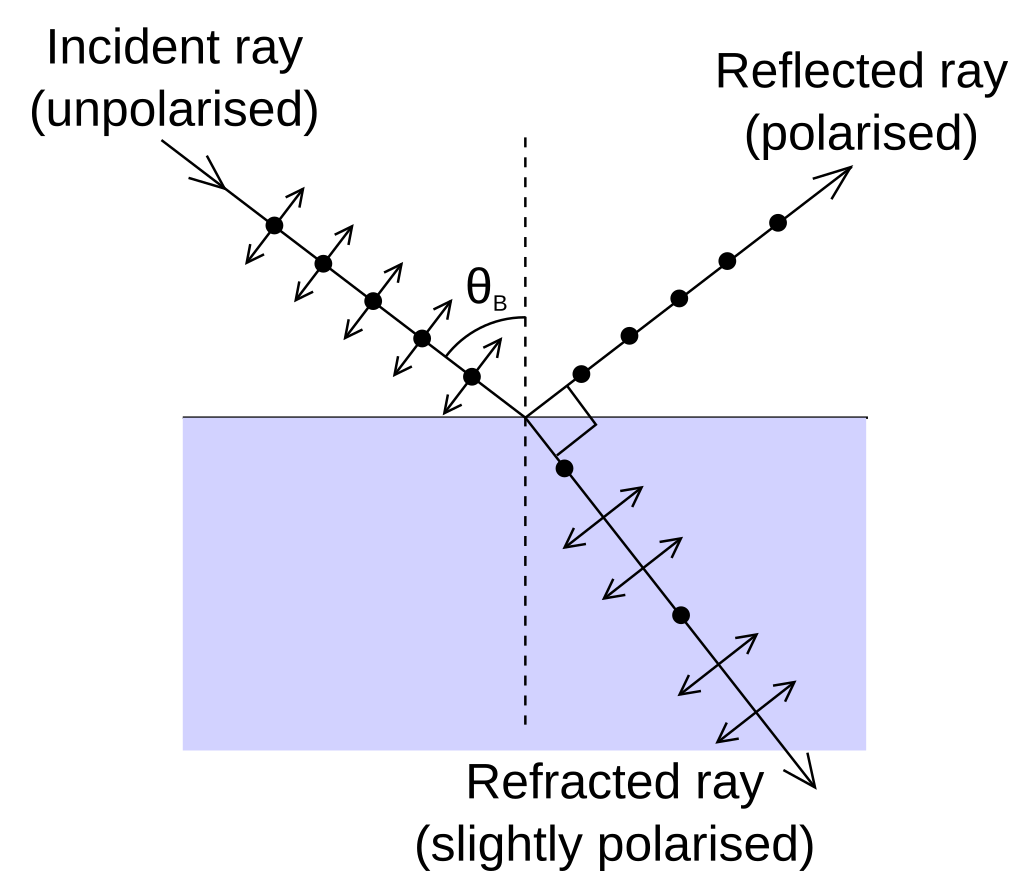
\includegraphics[width=0.6\textwidth]{figures/angulo_brewster.png} 
\end{figure}

\textcolor{red}{\textbf{Solução:}}\\

Para polarização total da luz refletida (ângulo de Brewster), os raios refletido e refratado ficam perpendiculares:
\[
\theta_B+\theta_t=90^\circ.
\]
Pela lei de Snell, com $n_1\simeq 1$ (ar) e $n_2=n$ (vidro),
\[
n_1\sin\theta_B=n_2\sin\theta_t
\quad\Rightarrow\quad
\sin\theta_t=\frac{n_1}{n_2}\sin\theta_B.
\]
Como $\theta_t=90^\circ-\theta_B$, então $\sin\theta_t=\cos\theta_B$, logo
\[
n_1\sin\theta_B=n_2\cos\theta_B
\;\Rightarrow\;
\tan\theta_B=\frac{n_2}{n_1}=n
\;\Rightarrow\;
\theta_B=\arctan(n).
\]

A resposta correta é alternativa \colorbox{green!50}{\textbf{D}}.

\end{flushleft}

\begin{flushleft}
\textbf{\textcolor{blue}{\Large Quest\~ao 31 - IFPA 2018 Franjas Claras na Fenda Dupla}}\\
\noindent

\subsection{Quest\~ao 31 - IFPA 2018 - Franjas Claras na Fenda Dupla}

O número máximo possível de franjas claras no experimento da fenda dupla de Young para distância entre as fendas igual a 
$2{,}5$ vezes o comprimento de onda da luz incidente é

\begin{itemize}
\item[(A)] 1.
\item[(B)] 3.
\item[(C)] 5.
\item[(D)] 7.
\item[(E)] 9.
\end{itemize}

\vspace{0.5cm}

\textcolor{red}{\textbf{Solução:}}\\[2mm]

Máximos de interferência: 
\[
d\sin\theta = m\lambda \quad (m\in\mathbb{Z}),
\]
com a condição $|\sin\theta|\leq 1 \;\;\Rightarrow\;\; |m|\leq \frac{d}{\lambda}.
$

Dado $d = 2{,}5\,\lambda$, obtemos:
\[
m_{\max} = \left\lfloor 2{,}5 \right\rfloor = 2.
\]

Assim, o número total de franjas claras visíveis é:
\[
2m_{\max}+1 = 2\cdot2+1 = 5.
\]

A resposta correta é alternativa \colorbox{green!50}{\textbf{C}}.

\end{flushleft}

\begin{flushleft}
\textbf{\textcolor{blue}{\Large Quest\~ao 28 IFRS 2023 - Índice do quarto meio (refração e ângulo crítico)}}\\
\noindent

\subsection{Quest\~ao 28 IFRS 2023 - Índice do quarto meio (refração e ângulo crítico)}

Um raio de luz se propaga em um meio 1 ($n_1=1{,}5$) e sofre refração ao penetrar em um segundo meio com índice de refração igual a 
$2$, com um ângulo de incidência na interface meio 1-meio 2 igual a $60^\circ$. Posteriormente, esse raio refrata novamente em um terceiro 
meio, com um ângulo de refração igual a $\theta$ (onde $\sin\theta=0{,}25$). Ao incidir no quarto meio, o ângulo de incidência corresponde ao ângulo crítico, 
resultando em reflexão interna total.

\begin{figure}[!h]
\centering
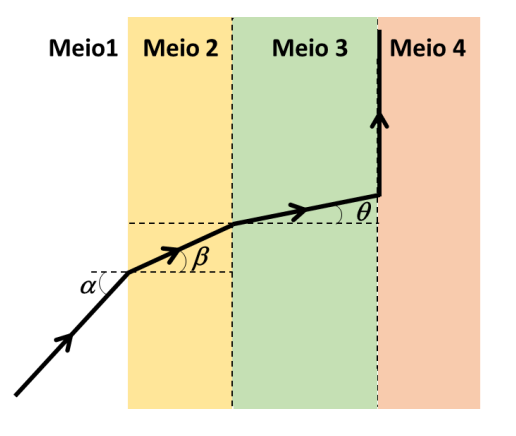
\includegraphics[width=0.5\textwidth]{figures/lei_snell.png} 
\end{figure}

Qual é o índice de refração mais próximo para o quarto meio?

\begin{itemize}
\item[(A)] $\dfrac{3\sqrt{3}}{4}$
\item[(B)] $\dfrac{\sqrt{3}}{3}$
\item[(C)] $\sqrt{3}$
\item[(D)] $2\sqrt{3}$
\item[(E)] $3\sqrt{3}$
\end{itemize}

\vspace{0.5cm}

\textcolor{red}{\textbf{Solução:}}\\[2mm]

Na interface meio 1 $\to$ meio 2, pela lei de Snell:
\[
n_1\sin 60^\circ = n_2\sin\beta,
\]
logo
\[
\sin\beta=\frac{n_1}{n_2}\sin60^\circ=\frac{1{,}5}{2}\cdot\frac{\sqrt{3}}{2}
=\frac{3}{4}\cdot\frac{\sqrt{3}}{2}=\frac{3\sqrt{3}}{8}\approx 0{,}649519.
\]

Na interface meio 2 $\to$ meio 3, novamente Snell:
\[
n_2\sin\beta = n_3\sin\theta.
\]
Isolando $n_3$ e usando $\sin\theta=0{,}25$:
\[
n_3=\frac{n_2\sin\beta}{\sin\theta}
= \frac{2\cdot\left(\dfrac{3\sqrt{3}}{8}\right)}{0{,}25}
= \frac{\dfrac{3\sqrt{3}}{4}}{0{,}25}
= 3\sqrt{3}.
\]

Na interface meio 3 $\to$ meio 4 o ângulo de incidência é o ângulo crítico $\theta_c$, portanto
\[
\sin\theta_c=\frac{n_4}{n_3}.
\]
Como o ângulo de incidência é igual a $\theta$ e $\sin\theta=0{,}25$, temos
\[
n_4 = n_3\sin\theta = 3\sqrt{3}\times 0{,}25 = \frac{3\sqrt{3}}{4}.
\]

A resposta correta é alternativa \colorbox{green!50}{\textbf{A}}.

\end{flushleft}

\begin{flushleft}
\textbf{\textcolor{blue}{\Large Quest\~ao 30 IFRS 2023 - Lei de Malus}}\\
\noindent

\subsection{Quest\~ao 30 IFRS 2023 - Lei de Malus}

Considere um feixe de luz linearmente polarizada com densidade de energia por unidade de área \(I_0=1000\ \mathrm{W/m^2}\). 
A luz oscila a \(+20^\circ\) em relação à vertical. Encontra-se em sequência dois polarizadores lineares ideais: o primeiro 
tem eixo de transmissão a \(-25^\circ\) em relação à vertical e o segundo a \(+35^\circ\) em relação à vertical. Qual é a 
intensidade da luz que emerge do segundo polarizador?

\begin{itemize}
\item[(A)] \(125\ \mathrm{W/m^2}\)
\item[(B)] \(250\ \mathrm{W/m^2}\)
\item[(C)] \(375\ \mathrm{W/m^2}\)
\item[(D)] \(485\ \mathrm{W/m^2}\)
\item[(E)] \(960\ \mathrm{W/m^2}\)
\end{itemize}

\vspace{0.5cm}

\textcolor{red}{\textbf{Solução:}}\\

Aplicamos a Lei de Malus em cada polarizador. A intensidade transmitida por um polarizador ideal é
\[
I = I_{\text{incidente}}\cos^2\theta,
\]
onde \(\theta\) é o ângulo entre a direção de polarização da luz incidente e o eixo do polarizador.

1. Ângulo entre a polarização inicial \((+20^\circ)\) e o primeiro polarizador \((-25^\circ)\):
\[
\theta_1 = 20^\circ - (-25^\circ)=45^\circ.
\]
Assim, a intensidade após o primeiro polarizador:
\[
I_1 = I_0\cos^2 45^\circ = 1000\cdot\left(\frac{\sqrt{2}}{2}\right)^2 = 1000\cdot\frac{1}{2}=500\ \mathrm{W/m^2}.
\]

2. Após o primeiro polarizador a luz fica polarizada segundo o eixo do primeiro polarizador (\(-25^\circ\)). O ângulo entre esse eixo e o segundo polarizador \((+35^\circ)\) é
\[
\theta_2 = (-25^\circ) - (+35^\circ) = -60^\circ \quad\Rightarrow\quad |\theta_2|=60^\circ.
\]
Portanto a intensidade após o segundo polarizador:
\[
I_2 = I_1\cos^2 60^\circ = 500\cdot\left(\tfrac{1}{2}\right)^2 = 500\cdot\frac{1}{4}=125\ \mathrm{W/m^2}.
\]

\vspace{0.3cm}

A resposta correta é alternativa \colorbox{green!50}{\textbf{(A) 125 W/m\(^2\)}}.

\end{flushleft}

\begin{flushleft}
\textbf{\textcolor{blue}{\Large Quest\~ao 16 - IFSUL 2025 - Lei de Malus}}\\
\noindent

\subsection{Quest\~ao 16 - IFSUL 2025 - Lei de Malus}

No ver\~ao, um dos destinos mais procurados para desfrutar os benef\'icios da esta\c{c}\~ao \'e o litoral. 
Instrumentos importantes utilizados para observar com conforto ambientes litor\^aneos s\~ao os \'oculos escuros. 
Para qualificar a imagem observada, muitos desses dispositivos s\~ao incrementados com filtros polarizadores, 
os quais evitam a ofusca\c{c}\~ao causada pela luz refletida na superf\'icie da \'agua, devido \`a redu\c{c}\~ao na intensidade luminosa transmitida.  

Considere uma luz n\~ao polarizada, com intensidade \(I_0\), incidindo em uma sequ\^encia de 2 polarizadores, conforme a figura. 

\begin{figure}
\centering
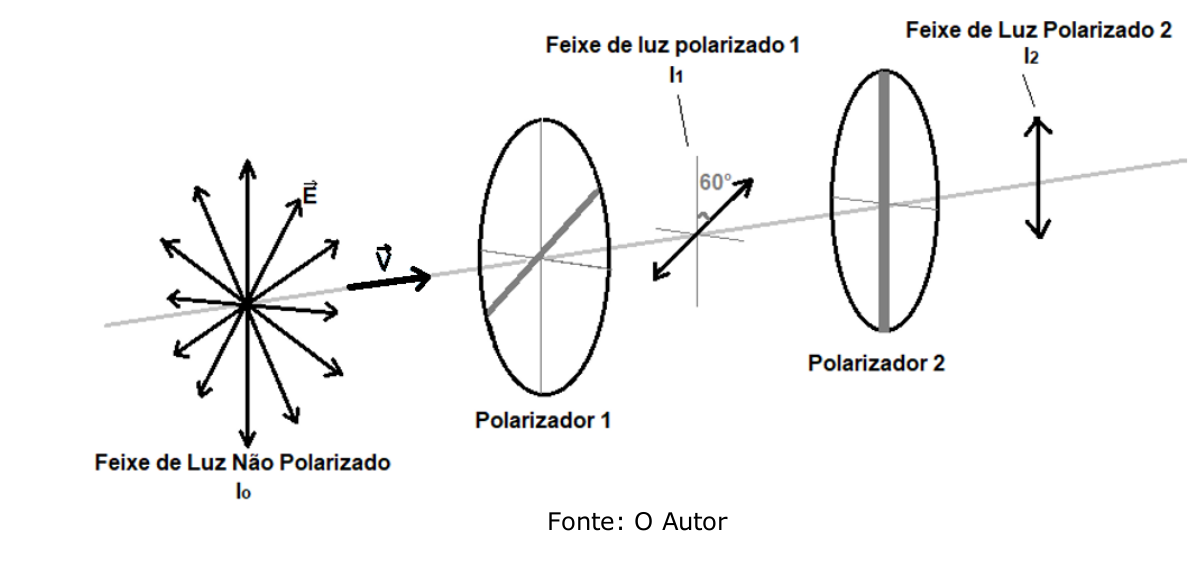
\includegraphics[width=0.6\textwidth]{figures/lei_de_malus.png}
\end{figure}

Qual das alternativas representa corretamente as intensidades dos feixes luminosos transmitidos pelos dois polarizadores (polarizador 1 e polarizador 2), respectivamente, sabendo que o \^angulo entre seus eixos \'e \(60^\circ\)?  

\begin{itemize}
\item[(a)] \(\tfrac{I_0}{2},\ \tfrac{I_0}{4}\)
\item[(b)] \(\tfrac{I_0}{2},\ \tfrac{I_0}{8}\)
\item[(c)] \(\tfrac{I_0}{4},\ \tfrac{I_0}{16}\)
\item[(d)] \(\tfrac{I_0}{4},\ \tfrac{I_0}{8}\)
\end{itemize}

\vspace{0.5cm}

\textcolor{red}{\textbf{Solução:}}\\

1. Quando a luz \textbf{n\~ao polarizada} incide em um polarizador ideal, a intensidade transmitida é reduzida pela metade:
\[
I_1 = \frac{I_0}{2}.
\]

2. Ap\'os o primeiro polarizador, a luz se encontra \textbf{polarizada linearmente}. Ao atravessar o segundo polarizador, aplica-se a Lei de Malus:
\[
I_2 = I_1 \cos^2\theta,
\]
onde \(\theta=60^\circ\).

3. Como \(\cos 60^\circ = \tfrac{1}{2}\), temos:
\[
I_2 = \frac{I_0}{2} \cdot \left(\frac{1}{2}\right)^2 
= \frac{I_0}{2} \cdot \frac{1}{4} 
= \frac{I_0}{8}.
\]

Portanto, as intensidades transmitidas pelos polarizadores 1 e 2 são, respectivamente:
\[
I_1 = \frac{I_0}{2}, 
\qquad 
I_2 = \frac{I_0}{8}.
\]

\vspace{0.3cm}

A resposta correta é a alternativa \colorbox{green!50}{\textbf{(b)}}.

\end{flushleft}

%\begin{flushleft}
%\textbf{\textcolor{blue}{\Large Quest\~ao - }}\\
%\noindent
%
%\subsection{Quest\~ao }
%
%\begin{itemize}
%\item[(A)] 
%\item[(B)] 
%\item[(C)]
%\item[(D)] 
%\item[(E)] 
%\end{itemize}
%
%\vspace{0.5cm}
%
%\textcolor{red}{\textbf{Solução:}}\\
%
%
%A resposta correta é alternativa \colorbox{green!50}{\textbf{...}}.
%
%\end{flushleft}